\chapter{Introduction} \label{introduction}
\begin{comment}
\begin{sectionplan}
     \begin{itemize}
          \item  General introduction about how important compilers are and how
                 everyone and is using them in some form or another.

          \item Talk about research into parallel compilers at a highlevel,
                ie the current state of research, when research has been done,
                parallel compilers historically of low importance.

          \item Justify further research into compilers based on their use
                in software development and other fields.

          \item Link to next section that describes how compilers work at a
                high level
     \end{itemize}
\end{sectionplan}
\end{comment}

A \gls{compiler} is an important part of the interface between a programmer
and the underlying hardware of a computer. The modern software ecosystem
could not exist without the frequent and extensive use of compilers in
the software development process. It is of no surprise that the study of
compilers and programming languages has been an important field of research
in computer science for many decades. Any improvements in compiler technology
can have wide and long lasting affects on software development as a whole
\citep{hall_compiler_2009}.

The focus of my \gls{fyp} is to study a subset of compiler research techniques
concerning aspects of parallel compilation. Research in this niche has been
historically of low priority. Traditional compiler architecture since the
1970’s has focused on minimizing memory use and optimizing for single threaded
performance. This was at a time when computers did not even have enough random
access memory to store all the data necessary for compiling large amounts of
source code. Commodity hardware has improved significantly since then. The
memory available in a computer is much more abundant than before and single
threaded processor speed is not improving at the same rate as it once did
\citep{shalf_future_2020, williams_whats_2017}. Nowadays, in fact, we are
seeing commodity processors comprising of several cores capable of running
dozens of processes concurrently. I believe this is sufficient cause to consider
alternative architectures that more efficiently utilize this environment. A
parallel compiler utilizes these methods of executing code in parallel in order
to speed up the compilation process.

Modern compilers in use today implement varying amounts of parallelism in order
to speed up compilation times. The \gls{rustc} compiler team reports a 50\%
performance improvement after making parts of the \gls{compiler_frontend} work
in parallel \citep{nicholas_nethercote_faster_2023}. Such improvements are not
limited to the \gls{compiler_frontend}. The mold \gls{linker} project boasts
significantly better performance than its competitors due to its extensive and
clever use of parallelism \citep{rui_ueyama_design_nodate}. The potential for
performance improvements is evident in modern compilers and tools. Moreover,
compiler research and development can generalize to other areas outside of
software development.

Applications of techniques traditionally associated with compilers can
be found in \gls{network_packet_parsing} \citep{wang_hyperscan_2019,
roesch_snort_1999} and \Gls{huffman_coding} in lossless image compression
\citep{howard_parallel_1996}. These areas, among others, can benefit from
research directed at improving compiler technology due to a significant
overlap in the underlying theory \citep{mytkowicz_data-parallel_2014}. Futher
development in compiler theory can benefit not only software development but
also tangential fields of research.

Before delving any further into parallel compilation, Section \ref{seq_comp}
will describe compilation in general, paying particular reference to the
traditional method of sequential compilation.

\section{Sequential Compilation} \label{seq_comp}
\begin{comment}
\begin{sectionplan}
     Short explanation of compiler technology and the structure of a compiler.
     Explain the compilation process and the use cases for compilation.
\end{sectionplan}
\end{comment}

\begin{figure}[t]
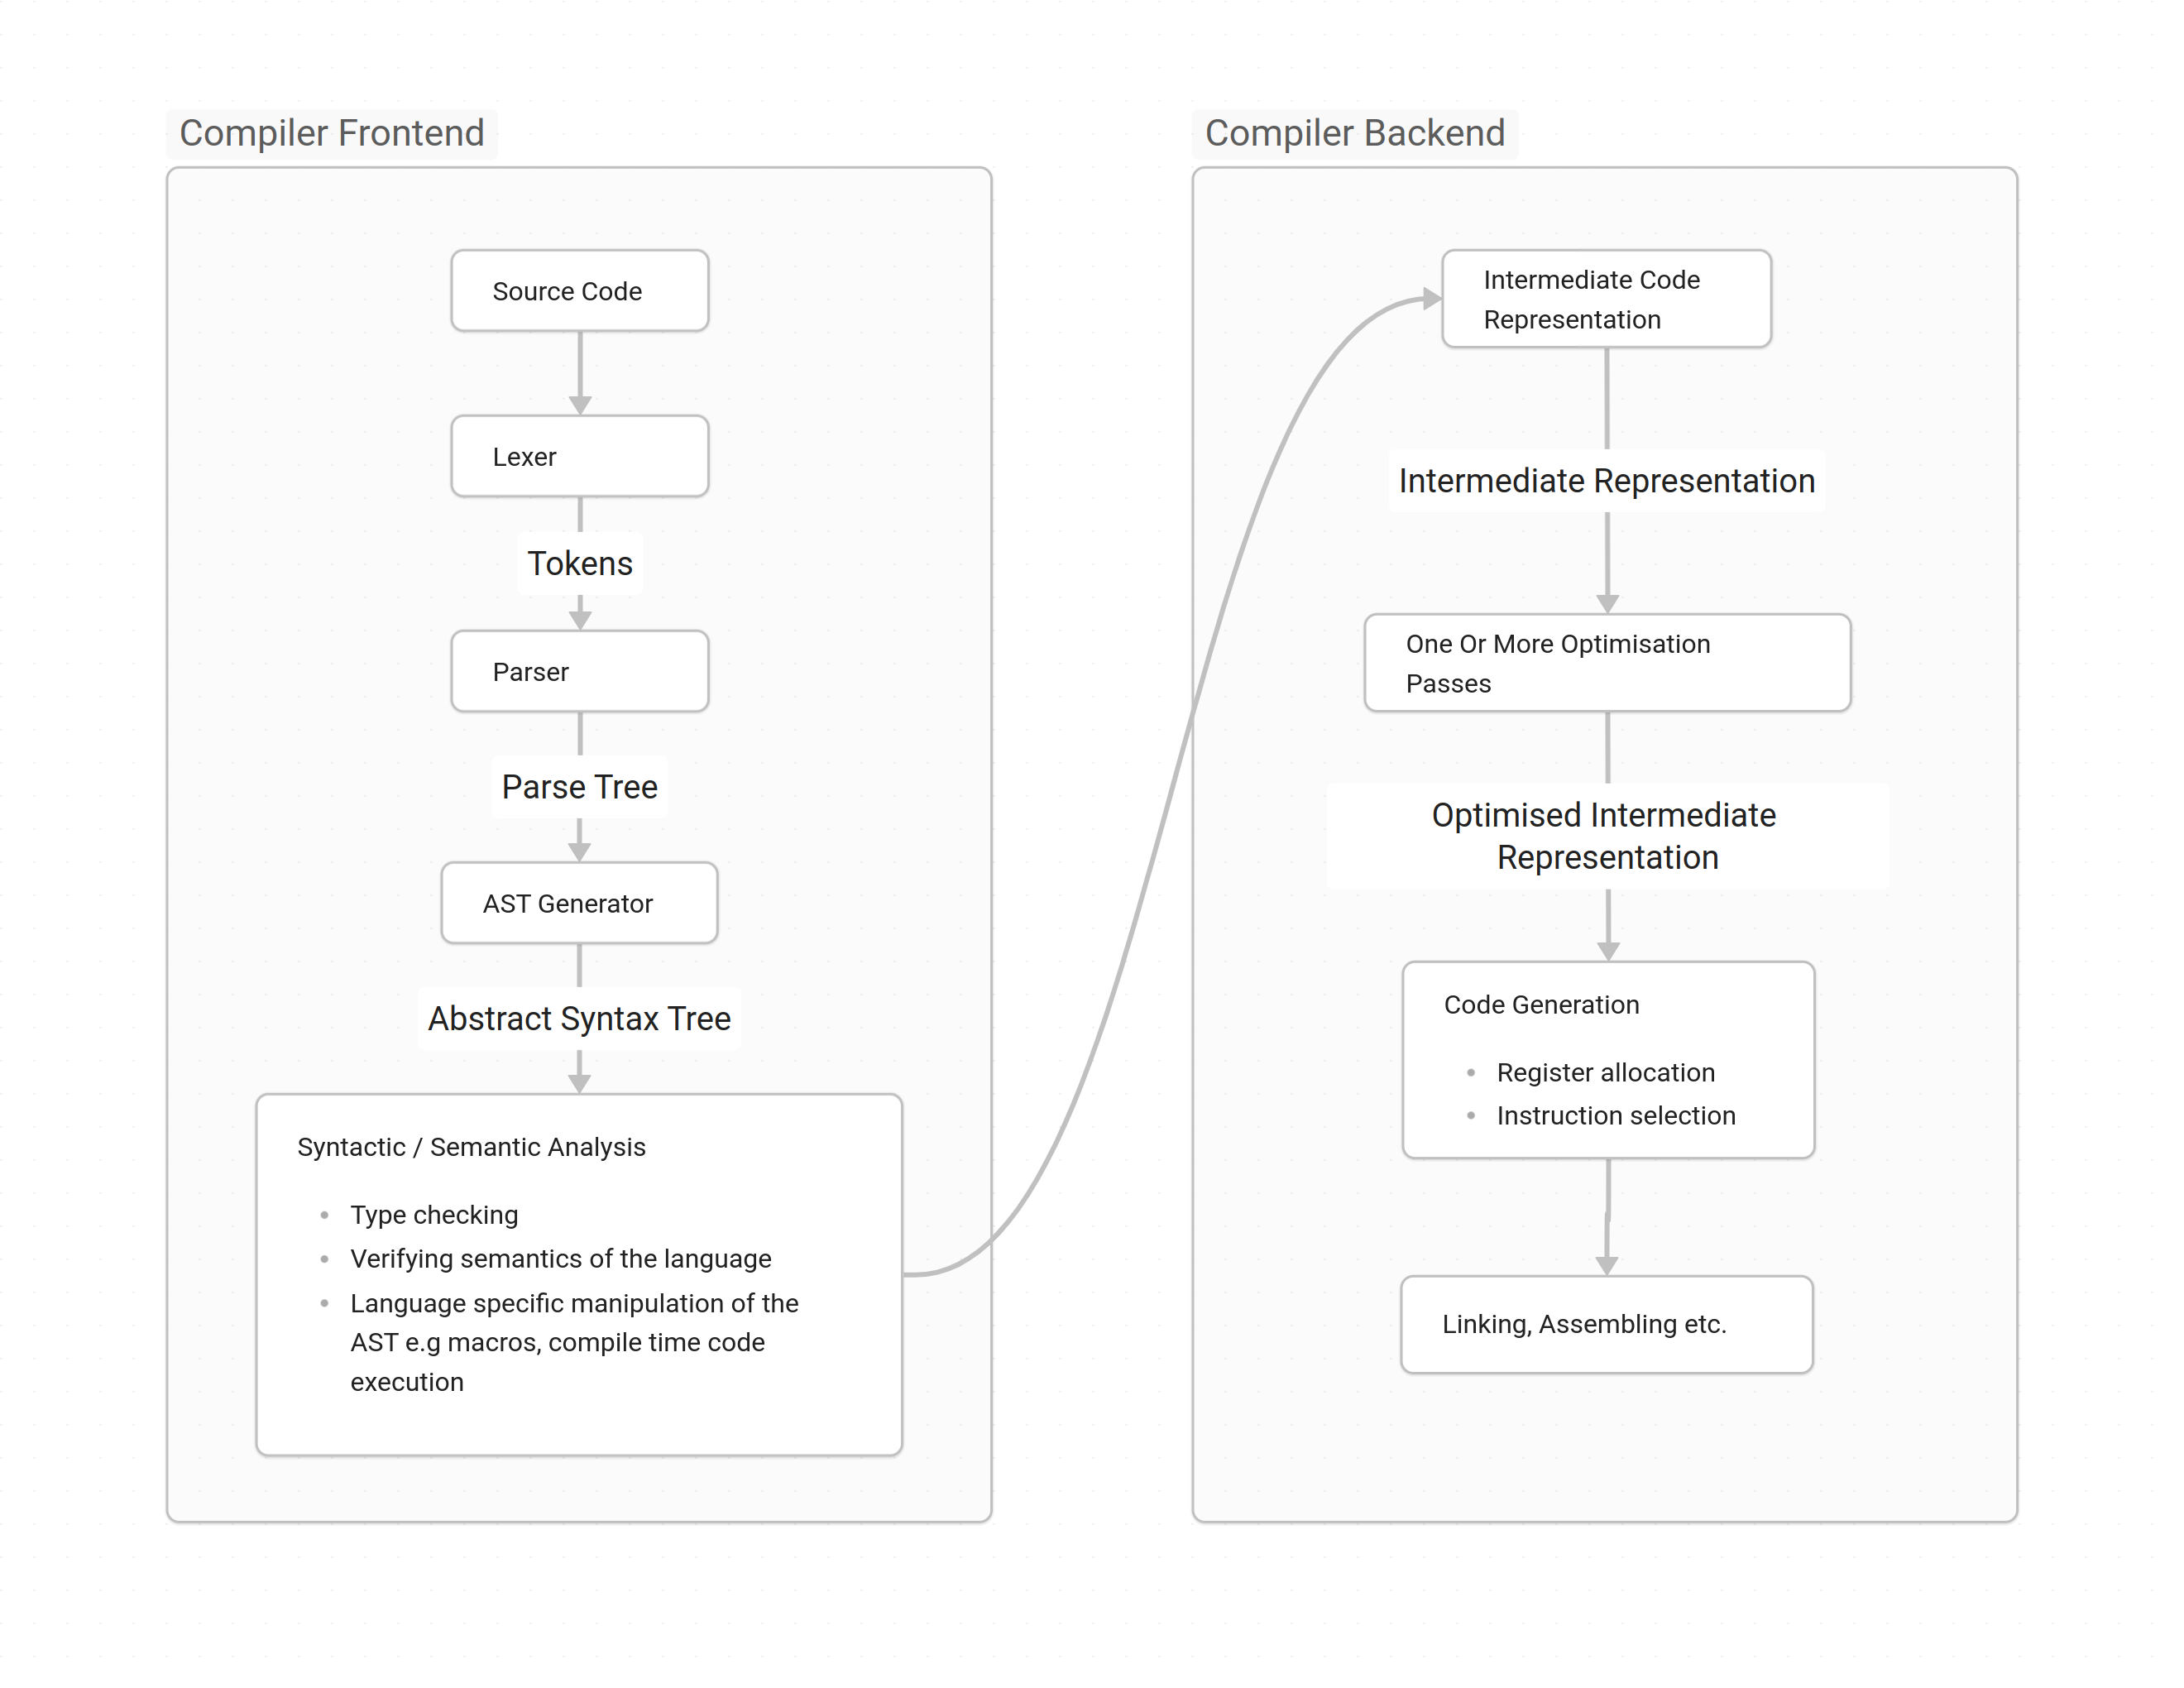
\includegraphics[width=\linewidth]{images/generic_compiler.png}
\centering
\caption{Compilation phases in a generic compiler}
\label{fig:compiler}
\end{figure}

Compilation is the process of translating a program written in a high-level
programming language into a semantically equivalent program written in a
lower-level programming language such as assembly or machine language. During
this process, a compiler will usually lose information in the source code that
is useful to the programmer but is useless to the machine that will ultimately
execute the program. Inside a compiler, the source code passes through several
algorithms that transform the code in various ways. These compilation stages are
shown in Figure \ref{fig:compiler}

The work of a compiler can be described as a multi-stage process resembling a
pipeline, where each stage works on the output of the previous stage thereby
producing the input for the next stage. The lexer splits the source code into
lexemes which are then tokenized for the next stage. In the parser stage, based
on the rules of the source language the code’s syntax is verified. During this
stage, an \gls{ast} is created, reflecting the hierarchy of the elements in the
code such as, tokens, variables and statements, and the relationships between
them. This AST is then analysed during the semantic analysis stage, considering
type checking, variable declaration prior to usage, unused variables and so
forth. The parts of the compiler up to this point are colloquially called the
frontend of the compiler.

These stages of compilation are often executed sequentially with each stage
doing the least amount of work necessary before passing control to the
subsequent stage. For example, the lexer will do only enough work to retrieve
the next token before passing that token to the parser. The parser will then
begin executing, doing as much work as it can with the input it got from the
lexer. Once it has done that, it might request more tokens from the lexer,
in which case control is returned to the lexer. This process repeats until
the entire contents of the source code in the input file has been processed.
Compiling in this way is much more memory efficient compared to performing
a compilation stage to completion prior to moving onto the next stage.
Difficulties with implementing this architecture using parallel processing
methods is described in Section \ref{compiler_parallel_methods}.

This type of architecture has traditionally been driven by a need to
optimize for memory use and single threaded performance. For example, in
the C programming language, programmers are forced to declare functions
before they are called. This was originally done to allow the compiler
to fully compile each function independently, without needing to keep all
the other functions in memory and avoiding a costly second pass over code
\cite{scott_programming_2015}. As a result of these decisions as well as
historical circumstances, the stages of a compiler that are responsible  for
taking a file containing source code to code generation are often implemented
with little to no parallelization. An example of going from source code to
machine code is the process of compiling a C file into an object file. As can be
seen from figure \ref{fig:compiler}, this envelopes a significant portion of the
compiler. The next section describes parallel compilation.

\section{Advantages of Parallel Compilation} \label{advantages_parallel_compilation}
\begin{comment}
\begin{sectionplan}
	What is meant by parallel compilation?

     Reasons why parallel compilation is good / better compared to sequential
	 compilation.

     \begin{itemize}
          \item More cores used during compilation increase compiler performance
                and better overall system usage

          \item Hardware investments in the industry involve specialisation
                and increasing reliance on performance gained from parallel
                architectures. Existing compilers cannot benefit from this.

          \item Choosing a language syntax as a language designer based on how
                well it can be processed in parallel in the future is necessary
                early on. Making those choices is difficult due to a lack of
                research.
     \end{itemize}
\end{sectionplan}
\end{comment}

Parallel compilation uses parallel processing methods in order to perform
various compilation stages at the same time. Parallel processing involves
executing more than one piece of code simultaneously. This can be achieved in
various ways depending on the available hardware. The most common of these
methods are reviewed in Section \ref{parallelisation_methods}. Potential ways
to structure a compiler that uses such methods is discussed in Section
\ref{compiler_parallel_methods}. This section considers the motivation for
performing various stages of compilation in parallel.

\subsection{Increased Compilation Speed with Additional Cores}

Using multiple \gls{cpu} cores during compilation can significantly speed
up compilation time. IBM researchers created an optimized lexer for a
machine that had a large number of cores that could run code in parallel
\citep{scarpazza_high-performance_2009}. It had eight \gls{cpu} cores where each
core could run eight threads in parallel for a total of 64 parallel threads.
More recent research into parallel lexing from 2014 achieved a 14 times speed
up for lexing HTML on a 16 core system \citep{mytkowicz_data-parallel_2014}.
Substantial performance gains can clearly be achieved through parallelization.
This shows how using parallel processing to speed up compilation tasks is not a
new idea.

\subsection{Parallel Compilation Research Aids Language Design}

For several programming languages, once their syntax goes into general
use, it becomes nearly impossible to reverse or change it, without breaking
programs already written in the particular language. This leads to programming
languages becoming complicated and difficult to define as new features
are added. For example, languages like C++ are very difficult to compile
sequentially, let alone in a parallel manner \citep{noauthor_most_2022,
noauthor_difficulties_nodate}. Research into and the development of parallel
compilers can aid future developers when they are choosing their syntax or
what features they want to implement without making their language difficult
to compile in parallel. \cite{barenghi_parallel_2015} demonstrate how this is
possible by, restricting the grammar of a language to an \gls{opg}.
It is currently rather difficult to design a language that can easily be
compiled in parallel due to a lack of research and prior work as compared to
sequential approaches.

\section{Advantages of Data-Parallel Compilation} \label{advantages_of_data_p_comp}
\begin{comment}
\begin{sectionplan}
	Justify looking at alternative forms of parallelism besides the status quo 	
	method of compiling source files in parallel and linking them together in the
	end.

	\begin{itemize}
     	\item Finer grained parallelism is better suited for running code on 				
			  massively parallel hardware like GPU's.

     	\item Error handling potential improved by being able to independantly
			  process any part of text. No need for complex parser recovery.

     	\item More parts of a program can be compiled in parallel which makes
			  better use of a computers parallel processing facilities. Mention 
			  ahmdals law.

		\item Significant speedups in other fields where only one stage of is 
			  needed like lexing and parsing very large amounts of structured 
			  data. Mention PAPAGENO parser with relation to simdjson.
	\end{itemize}
\end{sectionplan}
\end{comment}

Several current compilers can operate in parallel by compiling several source
code files at the same time. In this work I am looking at methods employing
\gls{data_parallel} techniques where various stages of a compiler can be executed in
parallel when compiling the same file. Due to a lack of prior work comparing
the two approaches directly, it is difficult to make an objective statement
regarding which approach is better. I will instead focus on the potential
advantages and disadvantages of using such a fine-grained approach.

\subsection{Parser Error Recovery}

An important responsibility of a compiler is to detect syntax errors and
present useful error messages to the programmer. Such syntax errors are often
detected during the parsing stage. An issue arises when a parser must then try
to continue parsing after encountering a syntax error. This parser recovery
process is frequently complicated and suboptimal \citep{medeiros_syntax_2018,
hutchison_pika_2020}. Certain parallel parsing algorithms, such as those
described in \citet{clarke_error_1993} and \cite{barenghi_parallel_2015}, allow
a compiler to forgo a complicated parsing recovery process by being able to
restart the parsing process immediately after encountering an error.

\subsection{Applications in Massively Parallel Computing}

There have been increasingly larger investments in the hardware industry for
specialized hardware beyond the typical \gls{cpu}.  For example, smart \glspl{nic}
 that offload network packet parsing from the \gls{cpu} or \gls{dpu} to provide
more facilities for networking and input/output related tasks than a typical
\gls{cpu}. A recent article from October 2023 outlined how the software stack
of \gls{amd} for general purpose computing on graphics cards known as \gls{rocm}
is now among their top priorities \citep{ward-foxton_rocm_2023}. As time goes
on, we are likely to see increasingly specialized and heterogenous hardware
\citep{stefan_lets_2021}.

Current compilation algorithms scale poorly on massively parallel hardware
such as \glspl{gpu}. This is due to the restrictions imposed on programs by
computing in such an environment. An approach utilizing \gls{data_parallel}
data structures described by \cite{hillis_data_1986} was applied by
\cite{voetter_compilation_2022} in order to create a parallel compiler
implementation that could run on a \gls{gpu}. This shows how  re-architecting
the compilation process makes it possible to execute a compiler in a massively
parallel environment, potentially achieving a linear performance increase that
scales with the number of available processing cores. This can only be achieved
by efficiently using \gls{data_parallel} techniques.

\subsection{Increased Performance in Individual Compilation Stages}

Data parallelism can massively improve the performance of various workloads
that utilise individual compilation stages. Tasks that involve processing large
amounts of data benefit the most. \cite{barenghi_parallel_2015} demonstrated
how \gls{json} parsing can be performed much faster using a parallel parser.
\cite{mytkowicz_data-parallel_2014} optimized a parallel regular expression
matching algorithm which has a large number of uses beyond lexical analysis.

\section{Project Objectives}

The goal of my \gls{fyp} is to research parallel compilation techniques for
a compiler frontend. In order to reach this goal, I intend to carry out a
literature review of exiting approaches in order to better understand the best
currently available techniques. Based on that literature review I will choose
a compiler frontend design, implement as much of it as time allows and evaluate
its performance. The compiler frontend will consist of the lexing, parsing and
semantic analysis stages.

\section{Structure of Report} \label{structure_of_report}

Chapter \ref{introduction} provides an introduction to compilers as well as
reasons to study parallel compilation methods.
\newline \newline
Chapter \ref{litreview} describes approaches for compiling
in parallel.
\newline \newline
Chapter \ref{design} will elaborate on the issues associated with designing a
parallel compiler, presenting suggested approaches from literature to overcome
these, prior to focusing on the compiler design and implementation decisions
specific to this work.
\newline \newline
Chapter \ref{implementation} explains the details of my implementation,
referring to aspects such as external code dependancies and program structure.
\newline \newline
Chapter \ref{evalandtesting} describes my testing methodologies and the
evaluation of my compilers performance.
\newline \newline
Chapter \ref{conclusion} concludes the report with a summary of the report and
concluding remarks.
